% !TeX root = main.tex
\section{Certification Schemes for Linear Programs} \label{sec:certification}

  In this section, we present examples of certification schemes for frequently arising problems such as computing the sum 
of values or functions that can be expressed as a linear programs. In the next section we will see the more general statement
about certification schemes for functions that satisfy a general Lipschitz continuity condition.

\subsection{Computing the Sum of Records} \label{ssec:certificationSum}

  One of the most basic certification tasks is computing the sum of the values of the records. For this task, we are given $n$ 
positive real numbers $x_1, x_2, \dots, x_n$ each one comming from a record in our data set. Our goal is to certify whether the
sum of all the records is closed to the sum of the subset of records that are valid, i.e. belong to $\Truth$. 

  More formally, we want to check with probability of failure at most $\delta > 0$ whether 
$\sum_{i \in \Workers} x_i \in \left[1 - \eps, \frac{1}{1 - \eps} \right] \cdot \sum_{i \in \Truth} x_i$ or there is at least 
one record $i$ such that $i \notin {\cal T}$. We show that there exists an efficient certification scheme for this task:

\begin{figure}[!h] \label{fig:certification sum}
  \centering
  {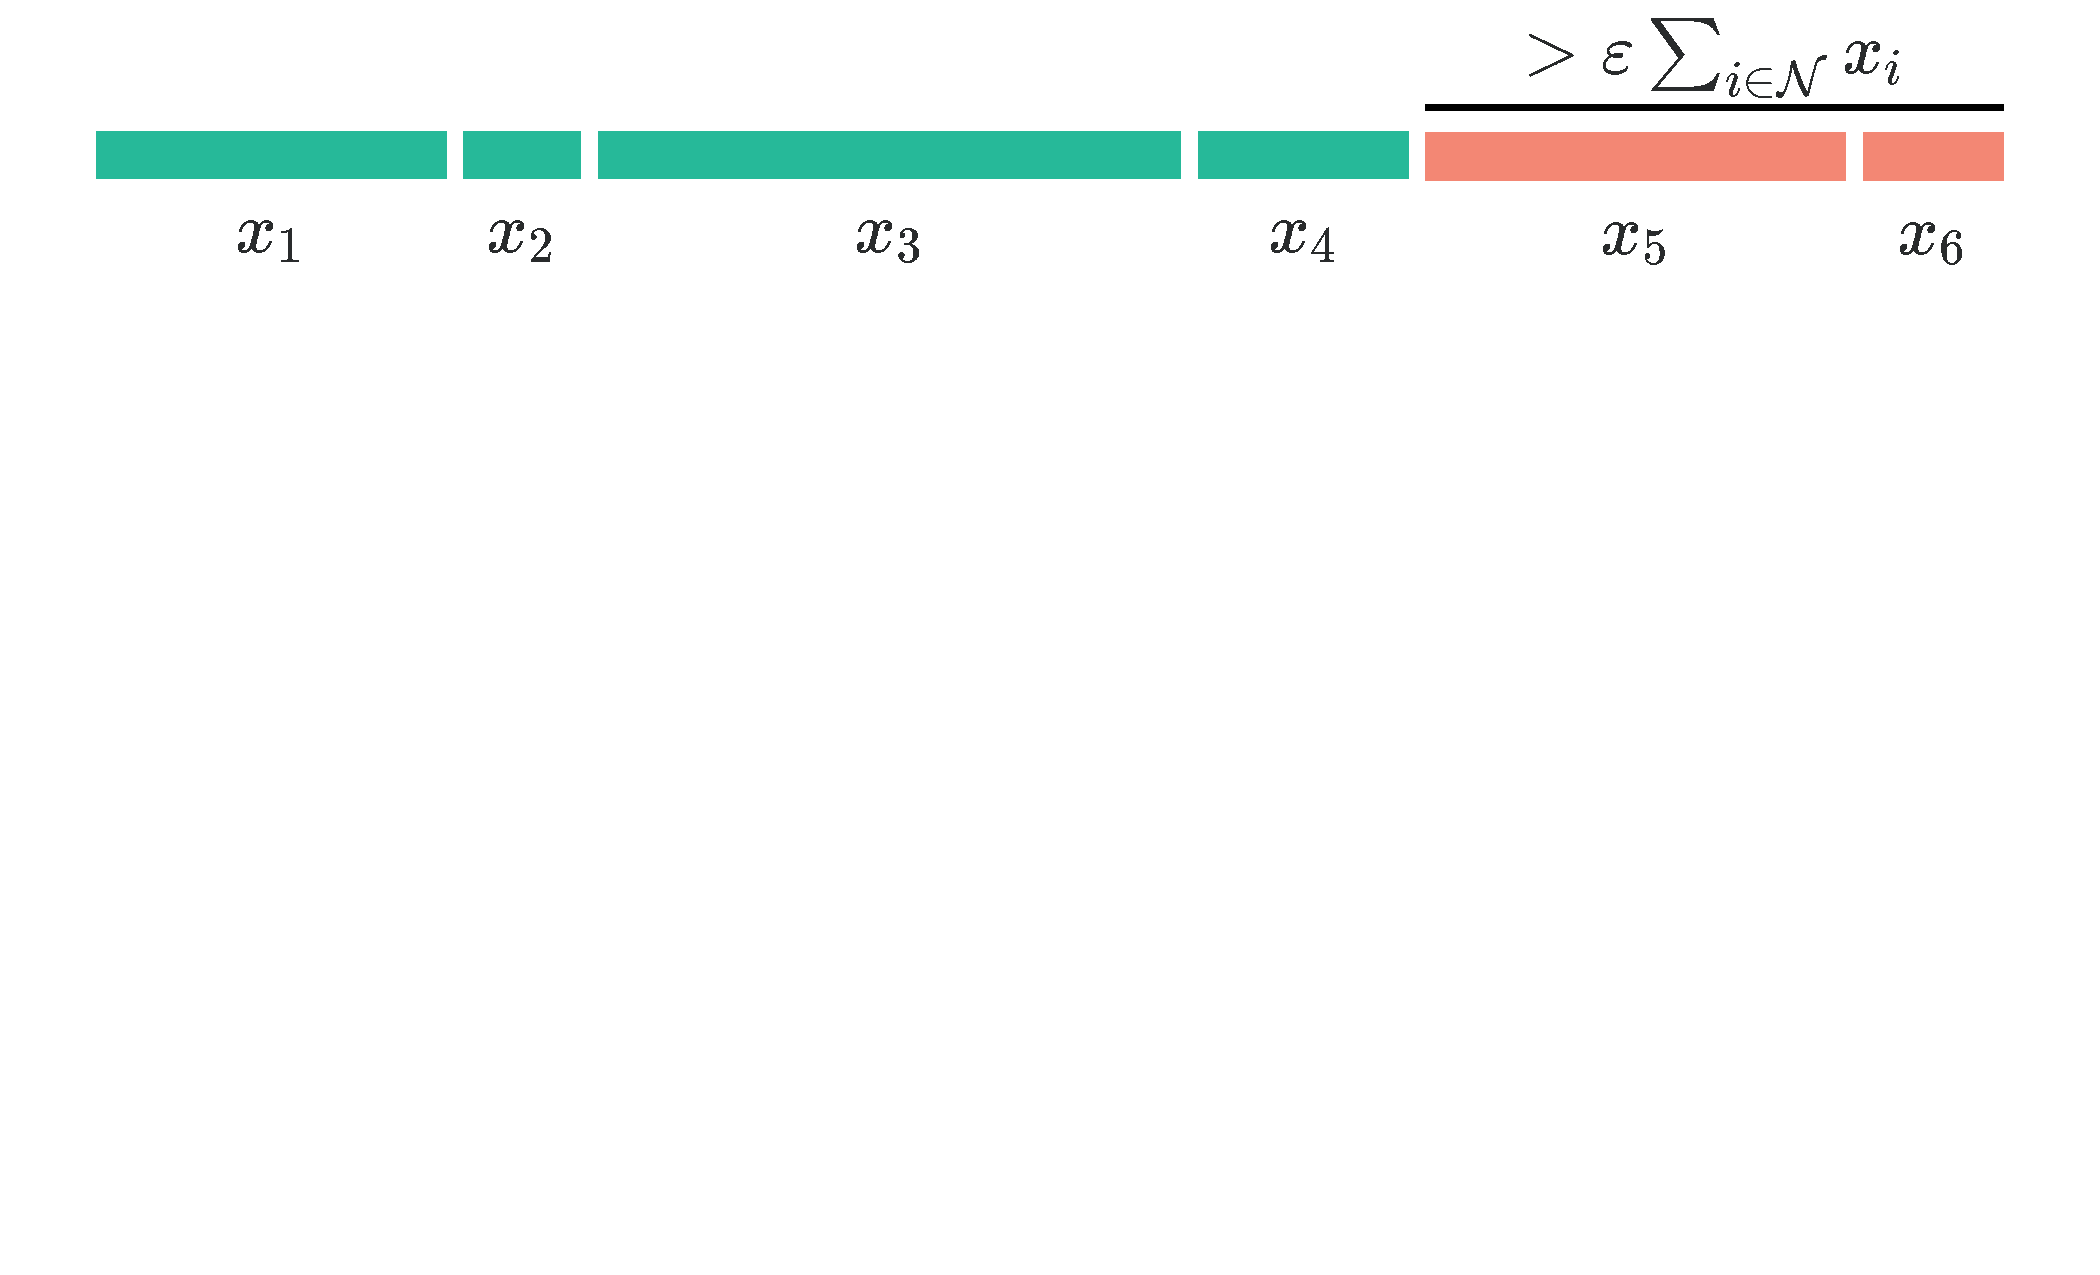
\includegraphics[clip, trim=1cm 17cm 2cm 0.2cm,width=0.65\textwidth]{figure4.pdf}}
  \caption{If the invalid records make up more than $\eps$ fraction of the total sum, there is at least $\eps$ probability that an invalid record is found with a single verification.}
\end{figure}


\begin{lemma}\label{lem:sumV}
Let $x_1, x_2, \dots, x_n \ge 0$ be the values of the records in $\Workers$ and $f(\xw) = \sum_{i \in \Workers} x_i$. Consider 
the probability distribution $p_i = \frac {x_i} {\sum_j x_j}$ which assigns to each record a probability proportional to its 
value $x_i$. Verifying $k=\Theta(\frac{1}{\eps}\log (1/\delta))$ records sampled independently from $p$, guarantees that the 
certification task succeeds with probability at least $1 - \delta$.
\end{lemma}

\begin{proof}
  Since $\Truth\subseteq \Workers$ and $x_i$'s are positive numbers, the inequality 
$\sum_{i \in \Workers} x_i \ge (1-\eps) \sum_{i \in \Truth} x_i$ holds trivially. If the inequality 
$\sum_{i \in \Workers} x_i \le \frac 1 {1-\eps} \sum_{i \in \Truth} x_i$ does not hold, we can bound the probability that all 
of the $k$ verifications fail to find an invalid record, as follows:

The probability that a single verification fails to find an invalid record is 
$\sum_{i \in \Truth} p_i = \frac {\sum_{i \in \Truth} x_i} {\sum_{i \in \Workers} x_i} < 1 - \eps.$

Therefore the probability that all $k$ verifications fail is at most $(1-\eps)^k$. Setting 
$k = \Theta(\frac{1}{\eps}\log (1/\delta))$, we guarantee that an invalid record is found with probability at least $1-\delta$.
\end{proof}

% !TeX root = main.tex

\subsection{Functions given by Linear Programs}
\label{ssubs:coverLP}

  We now extend the previous results for the sum function to more general objective functions that can be represented 
as linear programs. We first consider the special case of packing and covering LPs while later we present a result for
general linear programs.

$$
  \begin{array}{cc}
 	
\textbf{Packing LP} &
\textbf{Covering LP} \\
  
  \begin{array}{llll}
    \max_y  & \displaystyle\sum\limits_{i \in \Workers} c_{i} & y_{i} & \\
    \text{s.t.} & \displaystyle\sum\limits_{i \in \Workers} a_{ij} & y_{i} \le b_{j},  &j = 1, \dots, m \\
    & & y_i \ge 0, & i \in \Workers
  \end{array}
  
  &
  \begin{array}{llll}
      \min_x  & \displaystyle\sum\limits_{j = 1}^m b_{j} & x_{j} & \\
      \text{s.t.} & \displaystyle\sum\limits_{j = 1}^m a_{ij} & x_{j} \ge c_{i},  & i \in \Workers \\
      & & x_j \ge 0, & j = 1, \dots, m
    \end{array}
  \end{array}
$$

  Packing and Covering LP's are parameterized by the \emph{non-negative} parameters $a_{ij}, b_j, c_i$. We assume that
each record $i$ contains all parameters under his control, i.e. the value $c_i$ and $a_{ij}$ for all $j$, while the 
parameters $b_j$ are accurately known in advance.

  Packing LPs capture settings where several resources (each available in a quantity $b_j$) are to be divided among 
a set of agents in the system and agents report how much of each resource they need (given by $a_{ij}$) and how much
value they can generate if they are given the resources they ask for (given by $c_{ij}$). Our goal is to compute an
efficient allocation to agents that maximizes the total value generated. For the certification task, we want to 
certify that the total value generated by the true agents in an optimal allocation is close to the value computed 
under the possibly incorrect reports. We show that efficient certification schemes exist by extending the 
certification scheme presented for the sum function:

\begin{lemma} \label{lem:packingLP}
    Let $a_{ij}, c_i  \ge 0$ be values contained in the records $\Workers$ and $y^*$ be the optimal solution to the 
  packing LP. Consider the probability distribution $p_i = \frac {y^*_i c_i} {\sum_j y^*_j z_j}$ which assigns records 
  a probability proportional to their computed value $y^*_i c_i$. Verifying $k=\Theta(\frac{1}{\eps}\log (1/\delta))$ 
  records sampled independently from $p$, guarantees that the certification task for the packing LP succeeds with 
  probability at least $1 - \delta$.
\end{lemma}

  To see why this lemma holds, notice that the value $\sum_{i \in \Workers} c_i y^*_i$ computed using all the records 
$\Workers$ is higher than the value $\sum_{i \in \Truth} c_i \bar y_i$ computed using only the valid records $\Truth$. 
Moreover, if $\sum_{i \in \Truth} c_i y^*_i \ge (1-\eps) \sum_{i \in \Workers} c_i y^*_i$, then it must be that
$\sum_{i \in \Truth} c_i \bar y_i \ge (1-\eps) \sum_{i \in \Workers} c_i y^*_i$ as well, since setting $y_i = y^*_i$ 
for $i\in \Truth$ and $y_i=0$ otherwise is a feasible solution to the packing LP under the valid records. Finally, if  
$\sum_{i \in \Truth} c_i y^*_i < (1-\eps) \sum_{i \in \Workers} c_i y^*_i$, it means that invalid records contribute 
more than an $\eps$ fraction of the total value and thus an invalid record can be easily found as in the previous case
of the sum function.

  Covering LPs naturally capture various settings with public goods where the designer wants to introduce new goods to
satisfy all the demands coming from the records of our data set, but minimizing the total cost at the same time. In 
facility location problems, the designer wants to open facilities so that all a set of agents have access to at least
one facility and the agents report which locations are accessible to them.

  Certification schemes for covering LPs are less direct than previous examples, but can be easily obtained through LP 
duality. As the dual of a covering LP is a packing LP which has the \emph{exact same value}, we can use the certification 
scheme of Lemma~\ref{lem:packingLP} to certify that value. We directly get the following:

\begin{lemma} \label{lem:coveringLp}
    Let $a_{ij}, c_i \ge 0$ be values in the records $\Workers$. Verifying $k=\Theta(\frac{1}{\eps}\log (1/\delta))$ records 
  sampled independently according to a distribution $p$ given by the solution to the dual packing LP, guarantees that the 
  certification task for the covering LP succeeds with probability at least $1 - \delta$.
\end{lemma}

  General LPs can be written in the form of a packing or a covering LP but have arbitrary (possibly negative) parameters 
$a_{ij}, b_j, c_i$. The value of such LPs is harder to certify in general as a lot more verifications than before might be 
needed. However, we can show that $m$ verifications suffice to certify their value exactly.

\begin{lemma} \label{lem:generalLp}
    Let $a_{ij}, c_i$ be (possibly negative) values contained in the records $\Workers$. The certification complexity for 
  general LPs (written in the form of packing or covering LPs above) is at most $m$.
\end{lemma}

  To see why this is true, notice that in the covering LP formulation, the optimal value is given by at most $m$ tight 
constraints as there are only $m$ variables. Verifying the $m$ records relevant to those constraints guarantees that the 
optimal value of the LP under only the value of the records is equal to the computed one. This is because only those $m$ 
constraints determine the optimal value and even if every other constraint $i$ was dropped (i.e. because $i \notin \Truth$)
the value would remain the same. The result also holds for general LPs under the packing LP formulation by LP duality.

